\chapter{C/C++}
\label{sec:C/C++}
In der Vorlesung wurde mehr C als C++ gelehrt und gezielt auf fortgeschrittenen Konzepte wie Klassen, Exceptions, Templates, etc. verzichtet. 

\section{Command line arguments}
\subsection{C++ Programme bauen}\qquad\\
Ein Programm in C++ kann aus mehreren Header Dateien (*.h) und Quellcode Dateien (*.cpp) bestehen. Um diese zu einem Lauffähigen Programm umzuwandeln. Benötigt man einen Compiler wie g++. Dieser Besteht aus einem Linker, Preprocessor und dem Compiler selbst. \\
Der Preprocessor nimmt alle in den Sourcecode verlinkten Header Dateien und fügt diese zu 100 \% in den Sourcecode in dieser Stelle ein. Die Header Dateien können gleichzeitig in mehreren Sourcecode Dateien stecken. \\
Der Compiler wandelt anschließen die Sourcecode Dateien in Objectdateien um, welche vom Menschen nciht mehr gelesen werden können.\\
Der Linker fügt dann alle Object Dateien mit den verwendeten externen Bibiliotheken zu einem ausführbaren Programm zusammen.\\
\begin{figure}[h]
\centering
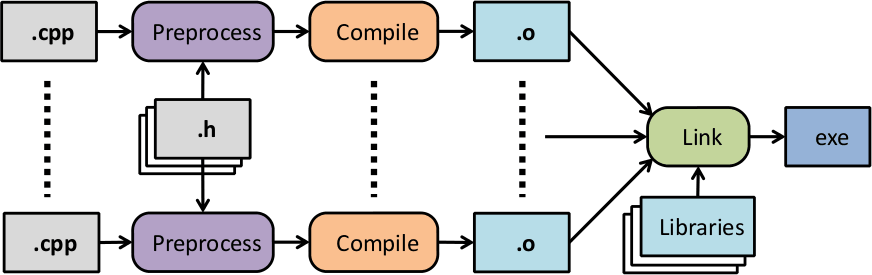
\includegraphics[width=0.75\linewidth]{mainmatter/pics/comp}
\caption[compiling]{C++ Programm Kompilieren}
\label{fig:comp}
\end{figure}
\subsubsection{Wozu dieses große Konstrukt?}
Viele Projekte enthalten eine sehr große Menge an Quellcode Dateien. Da man nicht bei jeder kleinen Änderung alle cpp Dateien neu in Objekt Dateien umwandeln will. Kann man auch schlicht nur die geänderten cpp Dateien durch den Preproccesor jagen und anschließend alle .o Dateien neu zu verlinken um die Änderungen zu testen. \\
Außerdem können vorhandene doppelte \#includes verhindert werden, indem man diese mit Guards definiert. Diese verhindern, dass die header Dateien, selbst bei mehrfacher Verlinkung, mehrfach in den Code einkopiert werden.
\begin{lstlisting}[language=Haskell]  
Datei: foo.h
#ifndef A_H
#define A_H
struct foo {
	int member;
};
void f(foo&);
...
#endif
\end{lstlisting}
Selbst wenn man nun diese header Datei in mehreren Dateien included, wird sie lediglich einmal hinzugefügt. Denn der Preprocessor, erkennt alle mit \# markierte Zeilen als seine an und führt das if entsprechend der Definition aus. Dabei geht der Guard von \#ifndef A\_H bis \#endif. Das \#define bedeutet, wenn A\_H noch nicht definiert wurde, definiere diese wie folgt. 
\section{I/O from console/file}	
\section{Control Statements and Loops}
\section{Call by Value / Call by Reference}
\section{Pointer}
\section{Memmory Management (Stack/Freestore)}
\section{Structs}
\section{Complex Data Structures (Lists, Trees)}
\section{Standard Containers and Algorithms}	

